\documentclass[conference]{IEEEtran}
\IEEEoverridecommandlockouts
\usepackage{cite}
\usepackage{amsmath,amssymb,amsfonts}
\usepackage{algorithmic}
\usepackage{graphicx}
\usepackage{textcomp}
\usepackage{xcolor}
\usepackage{tikz}
\usepackage{booktabs}
\usetikzlibrary{arrows.meta, positioning, fit, backgrounds}

% ---------------------------------------------------------------
% STATUS MARKERS: this draft is a working skeleton, not a submission-
% ready manuscript. \todo{} marks content that depends on work not
% yet done (implementation, experiments). Search for \todo before
% submitting -- none should remain.
% ---------------------------------------------------------------
\newcommand{\todo}[1]{\textcolor{red}{\textbf{[TODO: #1]}}}

\begin{document}

\title{Agentic AI-Based Multi-Agent Recommender System for Higher Education Decision Support}

\author{
\IEEEauthorblockN{Samuel Shine}
\IEEEauthorblockA{
Department of Computer Science (MCA)\\
CHRIST (Deemed to be University)\\
Bengaluru, India\\
samuelshine112003@gmail.com}
}

\maketitle

\begin{abstract}
Students choosing which university and program to apply to must jointly reason over
academic fit, career goals, financial constraints, location preferences, and employability
outcomes, typically before they have generated any interaction history a recommender can
learn from. Classical educational recommender systems address this pre-admission,
cross-institution decision using collaborative, content-based, or knowledge-based filtering,
but remain static, weakly explainable, and brittle under cold start. Recent agentic,
LLM-powered multi-agent recommenders address adaptivity, planning, memory, and
explainability, but published 2025--2026 systems apply these capabilities to
\emph{already-enrolled} students inside an \emph{already-chosen} program (academic
advising, learning-pathway sequencing, in-curriculum course selection) rather than to the
pre-admission choice itself. This paper identifies that intersection as an open gap,
proposes a five-agent architecture (profiling and constraint elicitation, retrieval,
multi-objective recommendation and planning, explanation, and memory-reflection) targeting
pre-admission cross-institution decision support, and lays out a research design --
research questions, hypotheses, and an evaluation protocol against classical baselines on
standard and agentic-specific metrics -- for the prototype currently under development.
\todo{Replace this paragraph with a results-bearing abstract once the prototype and
evaluation in Sections~\ref{sec:methodology}--\ref{sec:evaluation} are complete.}
\end{abstract}

\begin{IEEEkeywords}
agentic AI, multi-agent systems, recommender systems, higher education, large language
models, explainable recommendation, decision support
\end{IEEEkeywords}

\section{Introduction}
\label{sec:intro}

Choosing a university and program is a high-stakes, low-frequency decision made under
incomplete information. Prospective students must reconcile academic interests, career
goals, skills, financial constraints, location preferences, and employability outcomes,
usually without any prior interaction history a recommender system could exploit -- the
canonical cold-start setting. A substantial body of work addresses this decision with
collaborative filtering, content-based filtering, knowledge-based recommendation, and
hybrid or machine-learning classification approaches
\cite{hrspca,studieme,universityadmissionrecommendersystem,smartcollegeadmrecommendationsys,
userprofilinguniversityrecsys,contentbasedrecsys,multidmensionalrecsysuni,companalysisrecsys,
universityrecsyselahi,bertopicprogramrec}.
These systems established strong evaluation methodology, real datasets, and
education-specific features, but a 2024 systematic review of the space documents recurring
limitations: static recommendation pipelines, limited personalization, minimal conversational
interaction, weak adaptation over time, and weak explainability
\cite{recommendersyshighered}.

Separately, the emergence of large language model (LLM)-powered agents has produced a new
paradigm for recommendation: systems that plan, retrieve, reflect, and maintain long-term
memory across a conversation rather than scoring a fixed candidate set once
\cite{llmagentrecsyssurvey,agenticaisurvey,agenticaiarchitectures}. Agentic recommenders of
this kind have been demonstrated in e-commerce and general content domains
\cite{agenticaiframeworkrecommendersystem,multiagentrecommendersys,taurecbenchmark,
ragpersonalisedrecommendations}, and, more recently, in education -- but specifically for
students who are \emph{already enrolled} in an \emph{already-chosen} program: academic
advising Q\&A \cite{advisingwise}, in-program learning-pathway sequencing
\cite{agenticedurec}, and in-curriculum course selection \cite{onlinecoursemaskg}. None of
these systems address the earlier, arguably higher-stakes decision of \emph{which}
institution and program to choose in the first place.

This paper's central claim is that this earlier decision -- pre-admission, cross-institution
university and program selection -- is a distinct decision scope from the in-program
advising/pathway/course-selection problems that 2025--2026 agentic education systems solve,
and that it remains addressed only by pre-agentic methods. Section~\ref{sec:related}
substantiates this claim against the closest prior work in both the classical educational
recommender literature and the agentic recommender literature. Section~\ref{sec:architecture}
proposes a five-agent architecture for this gap. Section~\ref{sec:methodology} and
Section~\ref{sec:evaluation} lay out the research questions, hypotheses, and evaluation
protocol guiding the prototype and experiments currently under development.

This paper's contributions are:
\begin{enumerate}
\item An agentic multi-agent LLM architecture targeting pre-admission, cross-institution
higher-education decision support -- a decision scope distinct from the in-program
advising/pathway/course systems in recent agentic-education work (Section~\ref{sec:related}).
\item An explicit multi-objective reasoning mechanism integrating career goals, financial
constraints, location, and employability into agent planning, to be evaluated against
classical educational-RS baselines on both standard information-retrieval metrics and
agentic-specific metrics (explanation quality, adaptivity, cold-start robustness),
answering the "lack of educational evaluation frameworks" gap named explicitly in
\cite{llmagentrecsyssurvey}.
\item \todo{A working prototype and evaluation protocol, released as an open-source
artifact that third parties can run (repository URL to be added) -- finalize this claim
once Sections~\ref{sec:methodology}--\ref{sec:evaluation} are executed and the repository
is public.}
\end{enumerate}

\section{Related Work}
\label{sec:related}

\subsection{Classical educational recommenders for pre-admission decisions}

HRSPCA \cite{hrspca} and StudieMe \cite{studieme} are representative of the pre-admission,
cross-institution decision scope this paper targets: both recommend which
college/university a prospective student should consider, using hybrid collaborative
filtering with knowledge-based rules \cite{hrspca} or content-based TF-IDF similarity
\cite{studieme}. Somy\"urek and Aksoy \cite{multidmensionalrecsysuni} extend this to joint
university-and-major selection with a multidimensional recommender, the closest classical
match to the decision scope adopted here. Elahi et al.\ \cite{universityrecsyselahi}
develop a collaborative-filtering university recommender evaluated in two phases -- offline
cross-validation followed by an online user study measuring accuracy, diversity, perceived
personalization, satisfaction, and novelty -- an evaluation protocol this paper adopts as a
template (Section~\ref{sec:evaluation}). Lahoud et al.\ \cite{companalysisrecsys} compare
several such systems for major/career guidance and report fragmentation across methods
rather than a unified adaptive framework; El-Keiey et al.\ \cite{careerrecfeatureselection}
address the adjacent career-path decision with feature-selected machine-learning
classification over a public 20{,}000-record student-features dataset, and Hill et
al.\ \cite{bertopicprogramrec} recommend academic programs to prospective students via
BERTopic interest mining -- both from 2025, and both still single-model, non-agentic
pipelines. None of these systems reason via autonomous
planning agents, maintain memory across sessions, or generate grounded natural-language
explanations; Kamal et al.'s systematic review \cite{recommendersyshighered} confirms these
as recurring, unresolved limitations across the sub-field. By contrast,
\cite{serendipityuniversitycourserecsys} and \cite{recommendationsyscomplexconstraints}
address a related but distinct \emph{post-enrollment} scope (in-program course selection),
which this paper does not target.

\subsection{Agentic and multi-agent recommenders (general domain)}

Portugal et al.\ \cite{agenticaiframeworkrecommendersystem} propose an agentic multi-agent
recommender framework whose title closely resembles this paper's working title, making it
the closest general-domain precedent; it targets e-commerce recommendation and does not
incorporate educational features, datasets, or evaluation metrics. Yousefi Maragheh et
al.\ \cite{multiagentrecommendersys} survey multi-agentic design patterns for industrial
recommendation, and Narasimhan and Narasimhan \cite{taurecbenchmark} introduce a verifiable
benchmark for agentic recommenders, evaluated on general-domain conversational tasks across
five model families -- no education-specific agentic-recommendation benchmark yet exists.
Peng et al.'s survey \cite{llmagentrecsyssurvey} categorizes agentic recommendation into
recommender-oriented, interaction-oriented, and simulation-oriented paradigms and explicitly
identifies limited higher-education application as an open direction, which this paper
addresses directly.

\subsection{Agentic multi-agent systems in education}

Multi-agent educational recommenders predate LLMs: Marivate et al.\
\cite{humancapacitybuildingmas} deployed cooperative collaborative-filtering agents for
professional course selection in 2008, and Viswanathan \cite{adaptivemaselearning} surveys
the pre-LLM adaptive multi-agent e-learning line. The novelty claimed here therefore rests
on the combination of \emph{agentic LLM} capabilities (planning, memory, reflection,
grounded explanation) with the pre-admission decision scope -- not on multi-agent structure
alone. Three 2025--2026 systems are the decisive comparison set, since each combines
multi-agent LLM methods with an educational target. AdvisingWise \cite{advisingwise} is a
human-in-the-loop multi-agent system that answers academic-advising questions for
\emph{already-enrolled} graduate students within a fixed program, with all responses
validated by a human advisor before delivery -- it does not recommend which program to
choose, and its human-in-loop response drafting differs from autonomous multi-agent
planning. Chaturvedi and Gunawardena \cite{agenticedurec} deploy an 18-agent, four-tier
hierarchical architecture for adaptive in-program learning-pathway recommendation at
production scale (6{,}000+ users), but likewise address only \emph{post-enrollment}
curriculum adaptation. Zhong et al.\ \cite{onlinecoursemaskg} propose a three-agent
architecture (learner profiling, knowledge retrieval, recommendation generation) coupled
with a course knowledge graph for \emph{in-curriculum} course recommendation --
structurally the closest precedent to the architecture proposed in
Section~\ref{sec:architecture}, but scoped to course-level choice for enrolled students
rather than institution/program-level choice for prospective students, and without
multi-objective reasoning over career, financial, location, and employability constraints.

\subsection{Positioning}

Table~\ref{tab:gap} summarizes the resulting gap: no system in the surveyed literature
combines an agentic multi-agent architecture with the pre-admission, cross-institution
decision scope while reasoning jointly over the constraint set a prospective student
actually faces.

\begin{table}[t]
\caption{Positioning against the closest prior work}
\label{tab:gap}
\centering
\begin{tabular}{@{}p{1.6cm}p{1.5cm}p{1.6cm}p{1.5cm}@{}}
\toprule
\textbf{System} & \textbf{Target user} & \textbf{Decision scope} & \textbf{Method} \\
\midrule
\cite{hrspca}, \cite{studieme}, \cite{multidmensionalrecsysuni} & Prospective & Pre-admission, cross-institution & CF / CB / KB (pre-agentic) \\
\cite{advisingwise} & Enrolled & In-program advising & Multi-agent, human-in-loop \\
\cite{agenticedurec} & Enrolled & In-program pathway & Multi-agent (18+ agents) \\
\cite{onlinecoursemaskg} & Enrolled & In-curriculum course & Multi-agent + KG (3 agents) \\
\textbf{This work} & \textbf{Prospective} & \textbf{Pre-admission, cross-institution} & \textbf{Multi-agent LLM (5 agents)} \\
\bottomrule
\end{tabular}
\end{table}

\section{Proposed Architecture}
\label{sec:architecture}

The initial brainstorm for this project proposed seven agents (profiling, goal planning,
knowledge retrieval, recommendation, reflection, explanation, memory). Two of the closest
comparison systems bound a reasonable agent count: Zhong et al.\ \cite{onlinecoursemaskg}
report accuracy, recall, and F1 gains with only three agents, while Chaturvedi and
Gunawardena \cite{agenticedurec} use 18+ agents but only at production deployment scale
with a dedicated engineering team -- not reproducible within a single-author prototype.
This paper accordingly merges the original seven agents into five, keeping explanation and
memory-reflection as separate, visible components because they correspond directly to this
paper's headline claims (explainability, cold-start robustness via memory), while folding
goal-planning's constraint logic into profiling and recommendation.

\begin{figure}[t]
\centering
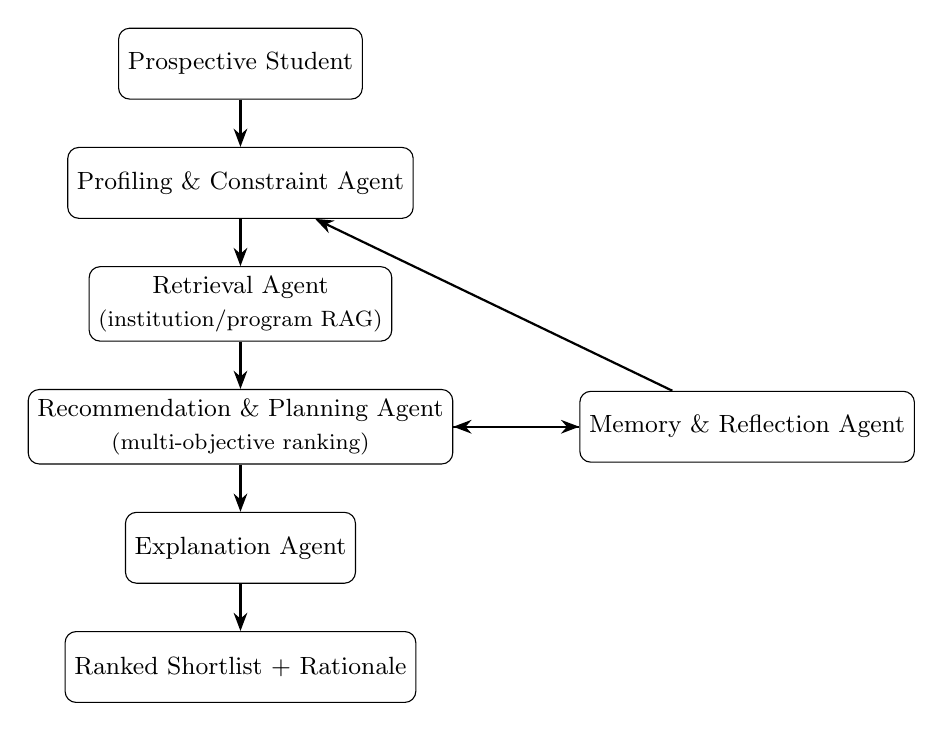
\begin{tikzpicture}[
  node distance=6mm and 8mm,
  box/.style={draw, rounded corners, align=center, minimum height=9mm, minimum width=28mm, font=\small},
  arr/.style={-Stealth, thick}
]
\node[box] (student) {Prospective Student};
\node[box, below=of student] (profile) {Profiling \& Constraint Agent};
\node[box, below=of profile] (retrieval) {Retrieval Agent\\[1pt]\footnotesize (institution/program RAG)};
\node[box, below=of retrieval] (recplan) {Recommendation \& Planning Agent\\[1pt]\footnotesize (multi-objective ranking)};
\node[box, below=of recplan] (explain) {Explanation Agent};
\node[box, right=16mm of recplan] (memory) {Memory \& Reflection Agent};
\node[box, below=of explain] (output) {Ranked Shortlist + Rationale};

\draw[arr] (student) -- (profile);
\draw[arr] (profile) -- (retrieval);
\draw[arr] (retrieval) -- (recplan);
\draw[arr] (recplan) -- (explain);
\draw[arr] (explain) -- (output);
\draw[arr] (memory) -- (profile);
\draw[arr] (recplan) -- (memory);
\draw[arr] (memory) -- (recplan);
\end{tikzpicture}
\caption{Proposed five-agent architecture. The Memory \& Reflection Agent persists the
student's constraint object across sessions and reviews the Recommendation \& Planning
Agent's shortlist before it reaches the Explanation Agent.}
\label{fig:architecture}
\end{figure}

\textbf{Profiling \& Constraint Agent.} Elicits academic background, career goals, and
financial, location, and employability-outcome constraints through structured dialogue;
outputs a structured student-constraint object consumed by downstream agents.

\textbf{Retrieval Agent.} Performs retrieval-augmented generation over institution and
program data (admissions criteria, cost, location, outcome statistics), following the
retrieval-plus-generation pattern established in \cite{ragpersonalisedrecommendations} but
against an education-specific knowledge base.

\textbf{Recommendation \& Planning Agent.} Ranks retrieved candidates against the
student-constraint object under multiple, potentially conflicting objectives (academic fit,
financial feasibility, location, employability outcome) -- the mechanism RQ2
(Section~\ref{sec:methodology}) evaluates directly.

\textbf{Explanation Agent.} Generates a per-recommendation natural-language rationale
grounded in the evidence the Retrieval Agent surfaced, addressing the explainability
limitation \cite{recommendersyshighered} documents in classical systems.

\textbf{Memory \& Reflection Agent.} Persists the student-constraint object and prior
shortlists across sessions, and reflects on the current shortlist before it reaches the
Explanation Agent -- the mechanism RQ3 evaluates for cold-start robustness.

\todo{This merge (7$\to$5 agents) is a judgment call, argued from buildability within a
one-month timeline, not derived from an ablation. Revisit after the ablation in
Section~\ref{sec:evaluation} (H3) -- if memory and reflection turn out to need separable
evaluation, they may need to split back into two agents.}

\section{Research Design}
\label{sec:methodology}

\subsection{Research questions}

\textbf{RQ1.} Does the architecture in Section~\ref{sec:architecture} improve
explainability and adaptivity over classical educational recommenders
(\cite{hrspca,studieme,multidmensionalrecsysuni}) while remaining within a 5\%
non-inferiority margin of their accuracy on standard recommendation metrics
(precision@$k$, recall@$k$, NDCG)?

\textbf{RQ2.} How should multi-objective constraints (academic fit, career goals,
financial constraints, location, employability outcomes) be represented and reasoned over
by specialized agents, compared to a single monolithic LLM prompt or a classical hybrid
scoring function?

\textbf{RQ3.} Do the Memory \& Reflection Agent's mechanisms measurably reduce cold-start
degradation for prospective students with no prior interaction history, compared to a
stateless agent pipeline?

\subsection{Hypotheses}

\textbf{H1.} The proposed architecture achieves higher user-perceived explanation quality
than a classical hybrid baseline re-implemented from \cite{hrspca,studieme}, while
remaining within a pre-registered 5\% \emph{relative} non-inferiority margin on
NDCG@$k$ (headline metric; precision@$k$ and recall@$k$ reported as secondary), on a
held-out admissions/preference dataset.

\textbf{H2.} Explicit multi-objective agent reasoning improves recommendation relevance
for students with conflicting constraints (e.g., financial limits vs.\ top academic fit)
relative to a single-objective ranking baseline.

\textbf{H3.} The Memory \& Reflection Agent mitigates cold-start degradation more
effectively than a stateless agent pipeline, measured across simulated first-session vs.\
later-session interactions.

\subsection{Planned methodology}
\label{sec:planned-methodology}

Evaluation uses a dual-dataset design (decided 2026-07-16, plan-mode dialogue; see
\texttt{chapter\_plan.md}): (i) the university-rating dataset of
\cite{universityrecsyselahi} (1{,}515 ratings, 80 users, 551 universities, plus metadata
for 12{,}003 crawled universities) as the primary accuracy benchmark for H1 -- real
preference data at exactly this paper's decision scope (requested from the authors;
request pending); and (ii) a synthetic constraint-preference dataset, seeded from the
public 20{,}000-record student-features corpus of \cite{careerrecfeatureselection} and
public program/admissions data following \cite{multidmensionalrecsysuni}, as the testbed
for H2 and H3 -- conflicting-constraint and multi-session cold-start conditions cannot be
expressed in rating-only data, and the scarcity of public educational datasets with such
structure is documented in \cite{slreducationalrecsys}. \todo{If the
\cite{universityrecsyselahi} data is not obtained in time, the synthetic dataset carries
H1 as well -- in that case state the self-constructed-benchmark limitation explicitly in
Section~\ref{sec:discussion}.}

\todo{Baselines (fidelity decision 2026-07-16: faithful re-implementation "as it was",
not library proxies): (a) a re-implemented hybrid CF+KB baseline following \cite{hrspca};
(b) a re-implemented content-based baseline following \cite{studieme}; (c) a single-prompt
LLM baseline (no multi-agent decomposition) to isolate the effect of the architecture
itself, following the ablation logic in \cite{onlinecoursemaskg}. Where the original
papers underspecify a detail, a best-faith reconstruction choice is made and logged in an
appendix reconstruction table. Prototype and experiments run on a local open-weights
Gemma model via Ollama (tag \texttt{gemma4:e4b}; \texttt{gemma4:12b} available for an
optional model-scale ablation); the released artifact is provider-agnostic
(bring-your-own API key or local model).}

\section{Evaluation Plan}
\label{sec:evaluation}

\textbf{Metrics.} The headline metric is NDCG@5 with graded relevance, under the
pre-registered 5\% relative non-inferiority margin against the strongest classical
baseline (H1); precision@5 and recall@5 are reported as secondary metrics, following
\cite{recommendationsys}. All systems are evaluated on the same held-out split of 100
students; the remaining 200 students serve as the historical pool for the HRSPCA
predictor stage.

\textbf{Explanation quality} is scored by LLM-as-judge on a three-dimension rubric
(clarity, groundedness in the provided program evidence, usefulness; 1--5 each),
following the protocol direction of \cite{advisingwise}. To avoid self-preference bias
-- same-family judges systematically inflate scores -- the judge is drawn from a
different model family than the experiment model (primary judge: Qwen-family 14B-class;
a Mistral-family second judge provides inter-judge agreement), with system identity
blinded and absolute rather than pairwise scoring to avoid position bias. LLM-as-judge
validity is treated as a limitation in Section~\ref{sec:discussion}.

\textbf{Conditions.} (i) the full five-agent pipeline; (ii) a \emph{no-memory} ablation
(H3); (iii) a \emph{single-objective} ablation collapsing the Recommendation \& Planning
Agent's reasoning to academic fit only (H2); (iv) a \emph{single-prompt} LLM baseline
replacing the five-agent decomposition, following the ablation logic in
\cite{onlinecoursemaskg}; and (v) the two re-implemented classical baselines. H1
comparisons use the full-information state (complete profile, mirroring the filled
application form classical systems assume); H3 uses the three-session
progressive-disclosure structure with simulated-user feedback reacting to what each
system actually recommended in the prior session.

\section{Results}
\label{sec:results}

\todo{This section reports completed runs only; agentic-condition rows are pending the
evaluation batches currently executing and MUST be filled from run records, never
estimated.}

\subsection{Top-$k$ accuracy (H1)}

Table~\ref{tab:results-h1} reports accuracy on the held-out 100-student evaluation
split at the full-information state. The re-implemented classical baselines
(Section~\ref{sec:planned-methodology}, reconstruction table in the appendix) set the
non-inferiority bar: the strongest baseline, HRSPCA, reaches NDCG@5 $= 0.793$, so under
the pre-registered 5\% relative margin the proposed system must reach NDCG@5 $\geq
0.753$ for H1's accuracy arm to hold.

\begin{table}[t]
\caption{Accuracy on the held-out evaluation split ($n=100$, full information).
Baseline rows are completed runs; remaining rows pending.}
\label{tab:results-h1}
\centering
\begin{tabular}{@{}lccc@{}}
\toprule
\textbf{System} & \textbf{NDCG@5} & \textbf{P@5} & \textbf{R@5} \\
\midrule
HRSPCA (re-impl.\ \cite{hrspca}) & 0.793 & 0.796 & 0.061 \\
StudieMe (re-impl.\ \cite{studieme}) & 0.673 & 0.760 & 0.113 \\
Single-prompt LLM baseline & \todo{pend.} & \todo{pend.} & \todo{pend.} \\
Five-agent (proposed) & \todo{pend.} & \todo{pend.} & \todo{pend.} \\
\bottomrule
\end{tabular}
\end{table}

\subsection{Explanation quality (H1), multi-objective conflict (H2), and cold start (H3)}

\todo{Explanation-quality rubric scores (both judges + agreement), the
single-objective ablation on the 162-student conflict subset (H2), and per-session
accuracy trajectories for full vs.\ no-memory conditions (H3) are pending their
respective batches. Report exactly what the run records and judge outputs contain;
where a hypothesis fails, report the failure (pre-committed in the evaluation design).}

\section{Discussion and Limitations}
\label{sec:discussion}

The gap argument in Section~\ref{sec:related} was verified against full-text readings of
the decisive prior work: all three agentic-education systems
\cite{advisingwise,agenticedurec,onlinecoursemaskg} were confirmed to address only
already-enrolled students (advising, learning pathways, course selection), and the two
re-implemented classical baselines \cite{hrspca,studieme} were confirmed to contain no
agentic, dialogue, or memory elements. Peripheral Cluster A citations remain verified at
the abstract level only.
The 7-to-5 agent merge (Section~\ref{sec:architecture}) is a buildability judgment, not an
empirical result, and may not survive the ablation in H3.

Beyond the gap-verification scope, this work carries the following limitations, stated
before results are in so that none can be read as post-hoc rationalization.

\textbf{Oracle circularity.} Ground-truth relevance in the synthetic dataset is a
published utility function fixed before any system was evaluated, not human judgment. A
system that reverse-engineered the formula would score perfectly. Mitigations: the
oracle is documented in the released dataset card, identical for all compared systems,
and H1's primary benchmark remains the real-preference dataset of
\cite{universityrecsyselahi} if access is granted; explanation quality is judged
independently of the oracle.

\textbf{Synthetic evaluation data.} The program catalog is fictional (real cities,
invented institutions, calibrated but invented economics), student constraints are
attached by documented sampling rules, and the three-session structure is scripted
rather than observed user behavior, with simulated-user feedback derived from the
oracle. Career coverage is IT-only, inherited from the seed corpus of
\cite{careerrecfeatureselection}; generalization beyond IT-bound students is untested.
The scarcity of public educational datasets motivating this choice is itself documented
\cite{slreducationalrecsys}.

\textbf{Baseline reconstruction fidelity.} Both classical baselines were re-implemented
from their papers' full texts, with every underspecified detail resolved by a logged
best-faith choice (appendix reconstruction table). Two original components could not be
expressed in the evaluation catalog (HRSPCA's college-capacity rule; StudieMe's
faculty-matching stage); both omissions remove hard filters and therefore favor the
baselines, not the proposed system.

\textbf{LLM-as-judge validity.} Explanation-quality scores come from LLM judges, not
human raters. Cross-family judging, blinding, absolute scoring, and two-judge agreement
reduce -- but do not eliminate -- known judge biases; no human-subject validation is
performed within this paper's timeline, and the judge scores should be read
accordingly.

\textbf{Single experiment model and scale.} All agentic conditions run on one local
open-weights model (\texttt{gemma4:e4b}); conclusions about the architecture are
conditioned on this model class. The evaluation split is $n=100$ students against a
200-program catalog -- larger than the closest classical baselines' user studies
\cite{universityrecsyselahi,bertopicprogramrec} but small in absolute terms.

\section{Conclusion and Future Work}
\label{sec:conclusion}

This paper identified pre-admission, cross-institution university and program selection as
a decision scope left unaddressed by both classical educational recommenders (pre-agentic
methods) and 2025--2026 agentic education systems (in-program scope only), proposed a
five-agent architecture for this gap, and laid out the research questions, hypotheses, and
evaluation protocol that will be executed next. \todo{Replace this paragraph with a
findings-bearing conclusion once Sections~\ref{sec:methodology}--\ref{sec:evaluation} are
complete.}

\section*{Acknowledgment}
\todo{No funding declared yet -- confirm funding/no-funding status before submission.}

\section*{Data Availability Statement}
The synthetic evaluation dataset (students, program catalog, graded relevance,
session structure), its generator, and its dataset card documenting provenance, the
ground-truth oracle, and known limitations are released with the paper's open-source
artifact. The public seed corpus of \cite{careerrecfeatureselection} is fetched from
its original GPL-3.0 repository at generation time and is not redistributed.
\todo{Add the artifact repository URL; if the \cite{universityrecsyselahi} dataset is
obtained and used for H1, state its on-request availability and usage conditions here.}

\section*{Author Contributions}
Single-author work; CRediT taxonomy roles apply in full to the sole author.

\section*{Conflict of Interest Statement}
The author declares no conflict of interest.

\section*{AI-Assisted Writing Disclosure}
\todo{This draft was produced with AI assistance (literature search, drafting, LaTeX
formatting) under author supervision. Replace with the venue-specific disclosure statement
required by the target IEEE conference before submission -- wording differs by venue.}

\bibliographystyle{IEEEtran}
\bibliography{references}

\end{document}
